\section{Liquidity, elimination and inheritance}
\label{sec:liquidity}

\subsection{Which eliminations could have been paid}

The cohort has 60 eliminations: 56 declarations and 4 automatic bankruptcies after a final mortgage. Fifty-nine estates pass to a player creditor and one to the bank. For each, we ask whether the debtor could have paid the debt that ended its game using only its own sales and mortgages, with no help, trade or future roll. The endpoint is narrow: paying the current debt does not imply surviving the next roll, and an unpayable debt says nothing about earlier choices.

\begin{figure}[htbp]
\centering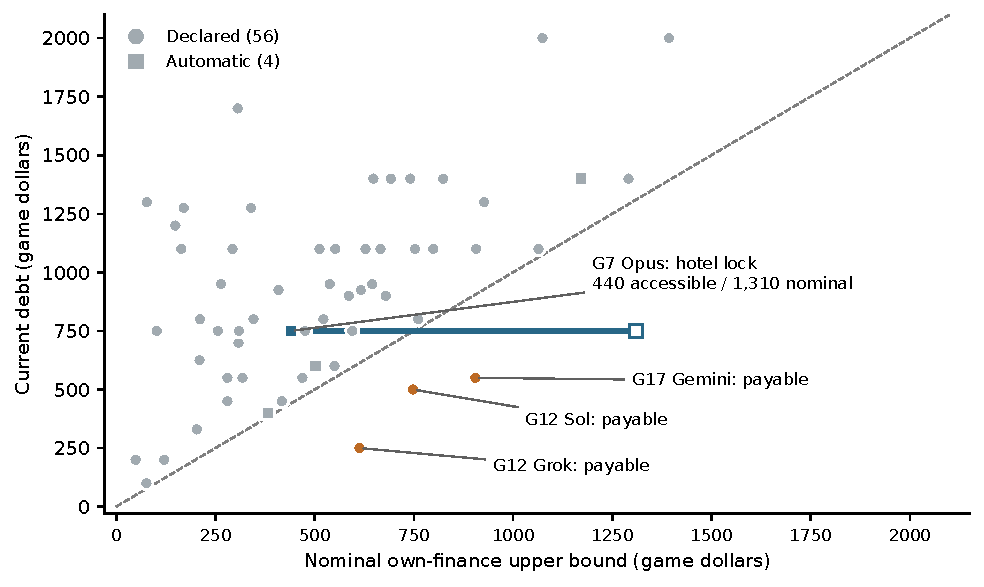
\includegraphics[width=0.94\linewidth]{financing.pdf}
\caption{Nominal own-asset upper bound (Equation~\ref{eq:upper}) against the debt for all 60 eliminations. Points left of the diagonal cannot be paid by any own-asset route. The three payable cases have executed payment witnesses. G7's open square marks its \$1,310 nominal bound and the filled square its proved accessible \$440. Other plotted bounds are not claimed to be reachable.}
\label{fig:financing}
\end{figure}

In 56 eliminations the generous upper bound $U$ is below the debt, so no own-asset route could pay (Figure~\ref{fig:financing}). Three eliminations were payable, and one was locked despite large nominal wealth (Table~\ref{tab:financing}).

\begin{table}[htbp]
\centering\small
\setlength{\tabcolsep}{4pt}
\begin{tabular}{@{}lllrrrrL{3.9cm}@{}}
\toprule
Case & Agent & Applied & Debt & Cash & Menu & Bound & Executed result\\
\midrule
G12 d190 & Sol & declare & \$500 & \$53 & \$183 & \$748 & Sales unlock red mortgages; pays with \$38 left.\\
G12 d249 & Grok & declare & \$250 & \$43 & \$43 & \$613 & Five house sales pay; \$43 left.\\
G17 d234 & Gemini & declare & \$550 & \$0 & \$30 & \$905 & Sales and mortgages pay; \$180 left.\\
G7 d339 & Opus & automatic & \$750 & \$390 & \$440 & \$1,310 & Exhaustive search: \$440 is the most reachable.\\
\bottomrule
\end{tabular}
\caption{The four eliminations not settled by the upper bound. ``Menu'' is cash plus every mortgage on the debtor's displayed liquidation menu; ``Bound'' is $U$ from Equation~\ref{eq:upper}. Witnesses are executed by the frozen certificate package and are neither minimal nor maximal; earlier checked routes leave \$8 and \$155 in the first and third cases.}
\label{tab:financing}
\end{table}

The three payable cases share a pattern. In each, the mortgages shown on the liquidation menu fall short of the debt, and selling buildings unlocks the rest, as salvage or by clearing a group so its deeds become mortgageable. Anyone who adds up the displayed mortgage options would call all three debts unpayable. The declarations themselves have different mechanisms. Sol's G12 d190 explanation omits the red collateral that house sales would unlock, and Gemini's G17 d234 explanation also understates accessible collateral. Grok's G12 d249 is different again: its content asks for a sale while the received call declares bankruptcy (Incident~\ref{inc:g12}).

G7 d339 runs in the other direction. Opus owes \$750 with \$390 in cash, one clear deed (Oriental, worth \$50 as a mortgage) and pinks at four houses, four houses and a hotel. The bank has no houses, so the hotel cannot be downgraded, and even-selling forbids selling a sibling's house first. The menu offers no building sale. Mortgaging Oriental triggers automatic bankruptcy at \$440. The player holds \$1,310 of nominal assets and can reach \$440 of them.

Staged financing also succeeds: in G20 d327--336 a player with \$49 sells \$700 of buildings and takes \$665 in mortgages to pay \$1,400. In G16 d602 the agent's note correctly totals \$1,393 against \$2,000, where an earlier research label had omitted \$160 of unlocked collateral, so the same test corrects analysts as well as agents.

\Incident{g12}{Bankruptcy applied while the response argues for selling (G12)}
\Setup{At G12 d249, Grok owes Opus \$250 in rent and has \$43. Its pinks hold two, two and three houses. The liquidation menu offers a building sale or a declaration and promises another decision after a partial sale.}

The assistant content requests a sale:

\TranscriptQuote{g12-sale}

The applied private note opposes bankruptcy:

\TranscriptQuote{g12_d249_private_final}

The one received tool call is \texttt{declare\_bankruptcy}, carrying this message:

\TranscriptQuote{g12_d249_public_bankruptcy}

\TranscriptFinding{The engine applies the declaration. No house is sold, and Grok's estate passes to Opus, which wins the game. An executed witness sells five houses and pays the \$250 with \$43 left. The two-house sale requested in content is legal but raises only \$100, reaching \$143; further sales would be needed.}

\TranscriptReading{This is a payable debt ending in an applied bankruptcy, and every text channel argues against the action that was applied. It is not evidence of deliberate surrender. The disagreement already exists in the non-streamed response received from the gateway, so it arose at or before that point; the records do not say whether generation, provider processing or the gateway produced it. The note's own arithmetic contains slips, so we rely on the executed route rather than the note.}

\TranscriptSource{G12 d249, turn 101, standard condition, selected attempt 0. The received tool array contains exactly one call. The witness is part of the frozen elimination package.}

\subsection{Spending and receipts}

The 103 spending units incur \$103,450 of own construction spending and collect \$93,000 in paid developed rent, \$92,550 of it after the owner's first purchase. Forty collect none, and 26 of those also trigger no elimination. These are realized flows, not returns: owners inherit buildings, rent depends on opponents' movement and survival, and unpaid terminal demands, salvage and estates are separate flows. Fifty-seven of the 60 eliminations arise from rent on developed groups, so a unit with little paid rent can still end an opponent's game. Successive owners of the same group can have opposite experiences. In G19 Opus spends \$1,200 on the dark blues, receives \$175 in developed rent and recovers \$600 in sales; Gemini inherits the deeds, spends \$2,000 and receives \$1,400. Appendix~\ref{app:offers} plots all 103 units.

\subsection{Creditor inheritance concentrates assets}
\label{sec:inheritance}

Under intact creditor inheritance, a bankrupt player's development and deeds pass to whoever it owes. The eventual winner is the estate recipient in 54 of 60 eliminations. Excluding the final elimination of each game, which hands everything to the last player by construction, the winner still receives 35 of 40 estates, 202 of 227 inherited deeds and \$7,148 of \$7,843 in estate cash. The winner also collects \$78,737 of the \$121,154 paid in rent. One estate (G13, Luxury Tax) goes to the bank.

These counts condition on the eventual winner, so they describe how assets concentrated; they do not estimate how much inheritance contributed to winning. Creditor identity, development, cash and landings evolve together. The records do show a recurring mechanism that matters for bargaining. A blocking or denial position lasts only as long as its holder stays solvent, and the blocker then passes to the creditor. Grok's G11 blocker came from Gemini's estate. In G18 Grok buys Illinois to keep Sol off the reds, and Illinois passes to Sol when Grok goes bankrupt to Sol eighteen turns later. In G13 the yellows that Opus paid to keep away from Sol pass to Sol at d311 (Incident~\ref{inc:g13}). In G2 the yellow group Sol finally completed passes to Gemini. Players also argue explicitly about who would inherit, which is the subject of the next section.

\FloatBarrier
